\begin{figure}
    \makebox[\linewidth][c]{
        \centering
        \begin{subfigure}{0.8\textwidth}
            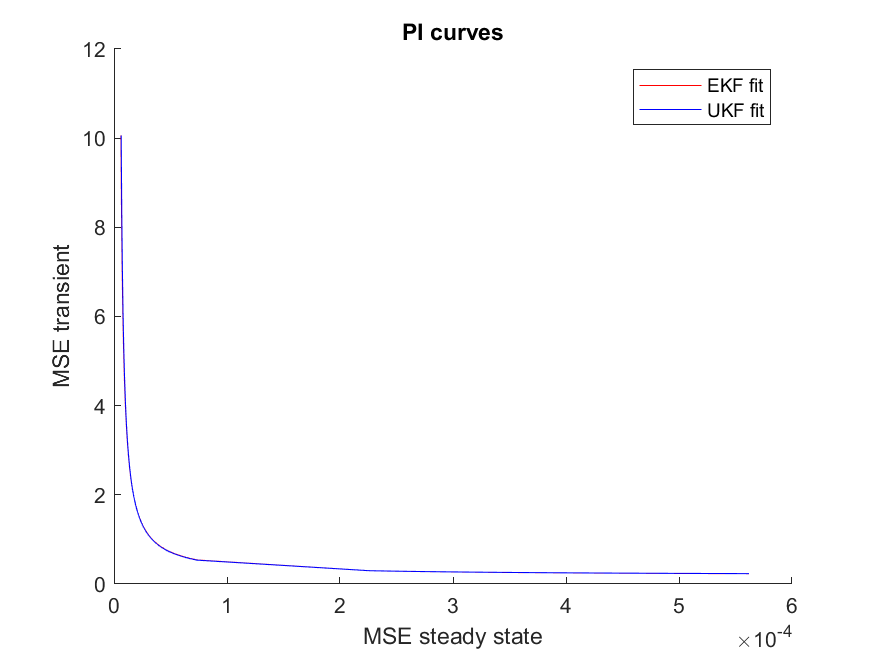
\includegraphics[width=\textwidth]{{images/results/pi/pi_fit_sn_0.005_sno0.000_q1.00e-06}.png}
            \caption{Our results. These have been obtained by a Least Square fit of a generic hyperbola $a+\frac{b}{x+c}$ over the raw data shown in Table~\ref{tab:pi_results}, $q=\num{1e-6}$, SNR 46 \si{\decibel}. $MSE_{\text{fit}} = \num{6.3e-3}$ }
            \label{fig:pi_fit}
        \end{subfigure}
        \begin{subfigure}{0.8\textwidth}
            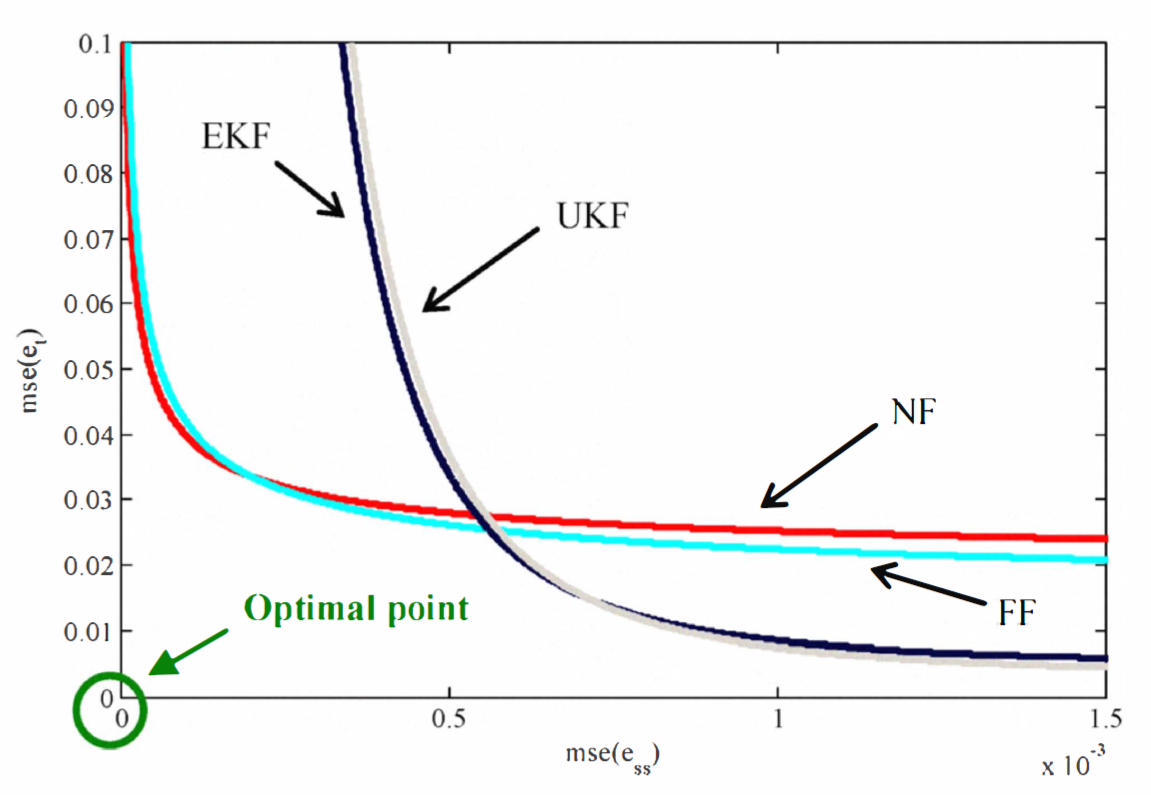
\includegraphics[width=\textwidth]{images/from_paper/pi_curves.png}
            \caption{Results from \cite[Figure~3]{UKF}}
        \end{subfigure}
        }
    \caption{PI curves comparison}
    \label{fig:results_comparison}
\end{figure}